\section{2020 年 11 月 23 日答疑记录}

幂函数、指数函数和对数函数相关的 ``图形过定点'' 问题, 一般是考虑利用恒等式
\[a^0=1\ (a\neq0),\quad \log_a 1=0\]
将函数中含参数的部分化为常数.

\begin{example}
    (1) 若 $a>0$ 且 $a\neq 1$, 求函数 $y=a^x+1$ 的图形所过的定点.
    
    (2) 若 $a>0$ 且 $a\neq 1$, 求函数 $y=\log_a x-1$ 的图形所过的定点.
\end{example}
\begin{solution}
    (1) 令 $x=0$ 知, 无论 $a$ 为何值, 总有 $y=2$, 即函数 $y=a^x+1$ 的图形过定点 $(0,2)$.
    
    (2) 令 $x=1$ 知, 无论 $a$ 为何值, 总有 $y=-1$, 即函数 $y=\log_a x-1$ 的图形过定点 $(1,-1)$.
\end{solution}

用类似的方法可以求得

$y=a^x-1$ 的图形过定点 $(0,0)$;

$y=2a^x+1$ 的图形过定点 $(0,3)$; 

$y=3a^{x-1}+3$ 的图形过定点 $(1,6)$; 

$y=\log_a (2x+1)+4$ 的图形过定点 $(0,4)$; 等等.

\begin{example}
    如图, 有一直角墙角, 两边的长度足够长, 在点 $P$ 处有一棵树与两墙的距离分别是 $a$\,m ($0<a<12$) 和 $4$\,m, 不考虑树的粗细. 现在想用 $16$\,m 长的篱笆, 借助墙角围成一个矩形的花圃 $ABCD$, 且将这棵树围在花圃内. 设此矩形花圃的最大面积为 $S= f(a)$ (单位: m$^2$), 则该函数的图形大致为 (\qquad).
        
    \begin{minipage}[c]{0.3\textwidth}
    \begin{center}
        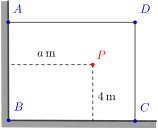
\includegraphics[scale=1]{2020-1208-1920-crop}
    \end{center}
    \end{minipage}
    \begin{minipage}[c]{0.7\textwidth}
        \small\centering
        \begin{tikzpicture}[scale=0.7]
          \draw[\myaxisarrow] (-0.7,0) -- (4,0) node[below] {$a$};
          \draw[\myaxisarrow] (0,-0.7) -- (0,3) node[left] {$S$};
          \draw (0,0) node[anchor=45] {$O$};
          
          \draw[line width=0.5pt] (0,2) -- (3,2);
          \draw (1.75,-1) node {(A)};
        \end{tikzpicture}\qquad
        \begin{tikzpicture}[scale=0.7]
          \draw[\myaxisarrow] (-0.7,0) -- (4,0) node[below] {$a$};
          \draw[\myaxisarrow] (0,-0.7) -- (0,3) node[left] {$S$};
          \draw (0,0) node[anchor=45] {$O$};
          
          \draw[line width=0.5pt,smooth,samples=100,domain=0:3] 
            plot(\x,{-(\x)^2 / 3 + 0.75*\x + 1.5});
          \draw (1.75,-1) node {(B)};
        \end{tikzpicture}\\
        \begin{tikzpicture}[scale=0.7]
          \draw[\myaxisarrow] (-0.7,0) -- (4,0) node[below] {$a$};
          \draw[\myaxisarrow] (0,-0.7) -- (0,3) node[left] {$S$};
          \draw (0,0) node[anchor=45] {$O$};
          
          \draw[line width=0.5pt] (0,2) -- (2,2);
          \draw[line width=0.5pt,smooth,samples=100,domain=1.98:3] 
            plot(\x,{-(\x)^2 / 3 + 0.75*\x + 1.83});
          \draw (1.75,-1) node {(C)};
        \end{tikzpicture}\qquad
        \begin{tikzpicture}[scale=0.7]
          \draw[\myaxisarrow] (-0.7,0) -- (4,0) node[below] {$a$};
          \draw[\myaxisarrow] (0,-0.7) -- (0,3) node[left] {$S$};
          \draw (0,0) node[anchor=45] {$O$};
          
          \draw[line width=0.5pt,smooth,samples=100,domain=0:3] 
            plot(\x,{-(3 - \x)^2 / 3 + 0.75*(3 - \x) + 1.5});
          \draw (1.75,-1) node {(D)};
        \end{tikzpicture}
    \end{minipage}

\end{example}
\begin{solution}
    设 $AB=x$\,m, 则 $CD=(16-x)$\,m. 因为矩形 $ABCD$ 要围住点~$P$, 所以
    \[\left\{\!\!\begin{array}{l}
        AD\geqslant a,\\
        DC\geqslant 4,
      \end{array}\right.\ \text{即}\quad
      \left\{\!\!\begin{array}{l}
        x\geqslant a,\\
        16-x\geqslant 4, 
      \end{array}\right.\ \text{解得}\quad
      x\in[a,12].\]
    设矩形 $ABCD$ 的面积为 $g(x)$, 则 $g(x)=x(16-x)$, $ x\in[a,12]$. 易知 $g(x)$ 是二次函数, 其 (完整) 图形的对称轴为 $x=8$. 由此可知,
    
    (1) 若 $0<a\leqslant 8$, 则 $g_{\max}= g(8)= 64$, 即 $S=f(a)=64$;
    
    (2) 若 $a>8$, 则 $g_{\max}= g(a)= a(16-a)$, 即 $S=f(a)=a(16-a)$.
    
    画出 $f(a)$ 对应的图形可知, 大致为 (C).
\end{solution}

